\chapter{Introduction}
Welcome to your remote lab for ECE 380, Introduction to Feedback Control.
The in-lab portion of this course was designed to give you a pseudo hands-on
feel for control using analog circuits. As this is a remotely delivered lab,
we no longer can provide you with the hands-on feel!

We persist. This lab is designed to run in MATLAB. You will engage
in understanding, developing, executing and analyzing Simulink
diagrams that model control systems. Every lab, though artificial, is
provided with brief motivation on how one can see this applied in a real
world problem. I hope this helps connect the abstract block diagrams of
Simulink with the real world.

Control systems is a very broad topic with a long history that even predates
the ideas discussed in this course. This course and lab covers the very basic
notion of control, the idea of the negative feedback loop, buttressed by
the mathematics of linear dynamical systems (Laplace theory).

\section{Logistics}
Please

\section{MATLAB and Simulink}
MATLAB is a desktop (or command line) numerical and symbolic
mathematics computing environment. We will not rely heavily on MATLAB
scripting itself and instead use Simulink. Simulink is a
package add-on to MATLAB that allows you to design and simulate
systems (physical or otherwise) using block diagrams like in
Figure~\ref{fig:intro:1}.
%
\begin{figure}
  \centering
  \begin{tikzpicture}[x=1in, y=1in]
    \node [draw, block] (Controller) {\(K_p + K_i\frac{1}{s}\)};
    \node [draw, block, right=0.5 of Controller] (Plant) {\(\frac{1}{s}\)};
    \node [draw, summer, left=0.5 of Controller] (Sum) {};
    \node [below=0.5 of Sum] (BelowSum) {};

    \draw [arrow, signal]
      (Controller.east) -- (Plant.west);
    \draw [arrow, signal]
      (Plant.east)
      --
      +(0.35, 0)
      |-
      (BelowSum.base)
      --
      (Sum.south)
      node [below right, annotate] {\(-\)};
    \draw [arrow, signal]
      (Sum.east) -- (Controller.west);
    \draw [arrow, signal]
      ($(Sum.west)+1*(-0.5, 0)$) -- (Sum.west);
    \draw [arrow, signal]
      (Plant.east) -- +(0.7, 0);
  \end{tikzpicture}
  \caption{
    Example feedback diagram. The blocks are differential equations, expressed
    as a Laplace transfer function, that take an input signal and produce an
    output signal.
  }
  \label{fig:intro:1}
\end{figure}
%
Figure~\ref{fig:intro:1} can be replicated perfectly in Simulink.
That fact makes it easy for engineers to quickly and easily design and verify
control designs. Simulink even supports direct interaction with
hardware but we will not utilize this feature.

The core of Simulink is the notion of a \emph{block}, maps that take an input
signal and produce an output signal.
The blocks we'll be concerned with primarily are \emph{gains}
(multiplier) depicted in Simulink like
\begin{center}
  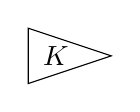
\begin{tikzpicture}[x=1em, y=1em]

    \draw
      (0, 0)
      --
      (3, 1)
      --
      (0, 2)
      --
      (0, 0)
      --
      (3, 1)
      node [at={(1, 1)}] {\(K\)};

  \end{tikzpicture}
\end{center}
and \emph{transfer functions} depicted in Simulink like
\begin{center}
  \begin{tikzpicture}[x=1em, y=1em]

    \node [draw, block] (Plant) {\(\frac{s+1}{s+2}\)};

  \end{tikzpicture}.
\end{center}
You will be provided template blocks to help you set up the Lab plant, the
system we wish to control, and it will be your task to analyze this block
design a controller, and implement it by linking up blocks to the plant
in the appropriate feedback architecture.

\section{Git Version Control}
We will be using the \texttt{git} version control system in tandem with
the Gitlab hosted on \url{git.uwaterloo.ca} to facilitate delivery of lab
content and to give you a mechanism for
\begin{enumerate}[label=(\arabic*)]
  \item{tracking your temporary work, and}
  \item{submitting your final work.}
\end{enumerate}
There is no requirement that you use git ``properly.'' If you are not
comfortable using the terminal to perform git operations, you can use graphical
tools like \href{https://www.sourcetreeapp.com/}{Sourcetree} or
\href{https://www.gitkraken.com/git-client}{GitKraken}. You can even manually
upload the files using the graphical web interface at \url{git.uwaterloo.ca}.
As long as your able to download files from your repository and upload your
solutions, I am happy. Having said that, it is an important skill in this
day and age to understand how to use version control. Therefore, this is a
great opportunity to learn git!
